
\chapter{CALock: A New Approach to Multi-Granularity Locking} \label{chap:calock}
\begin{figure}
	\centering
	\captionsetup{justification=centering}
	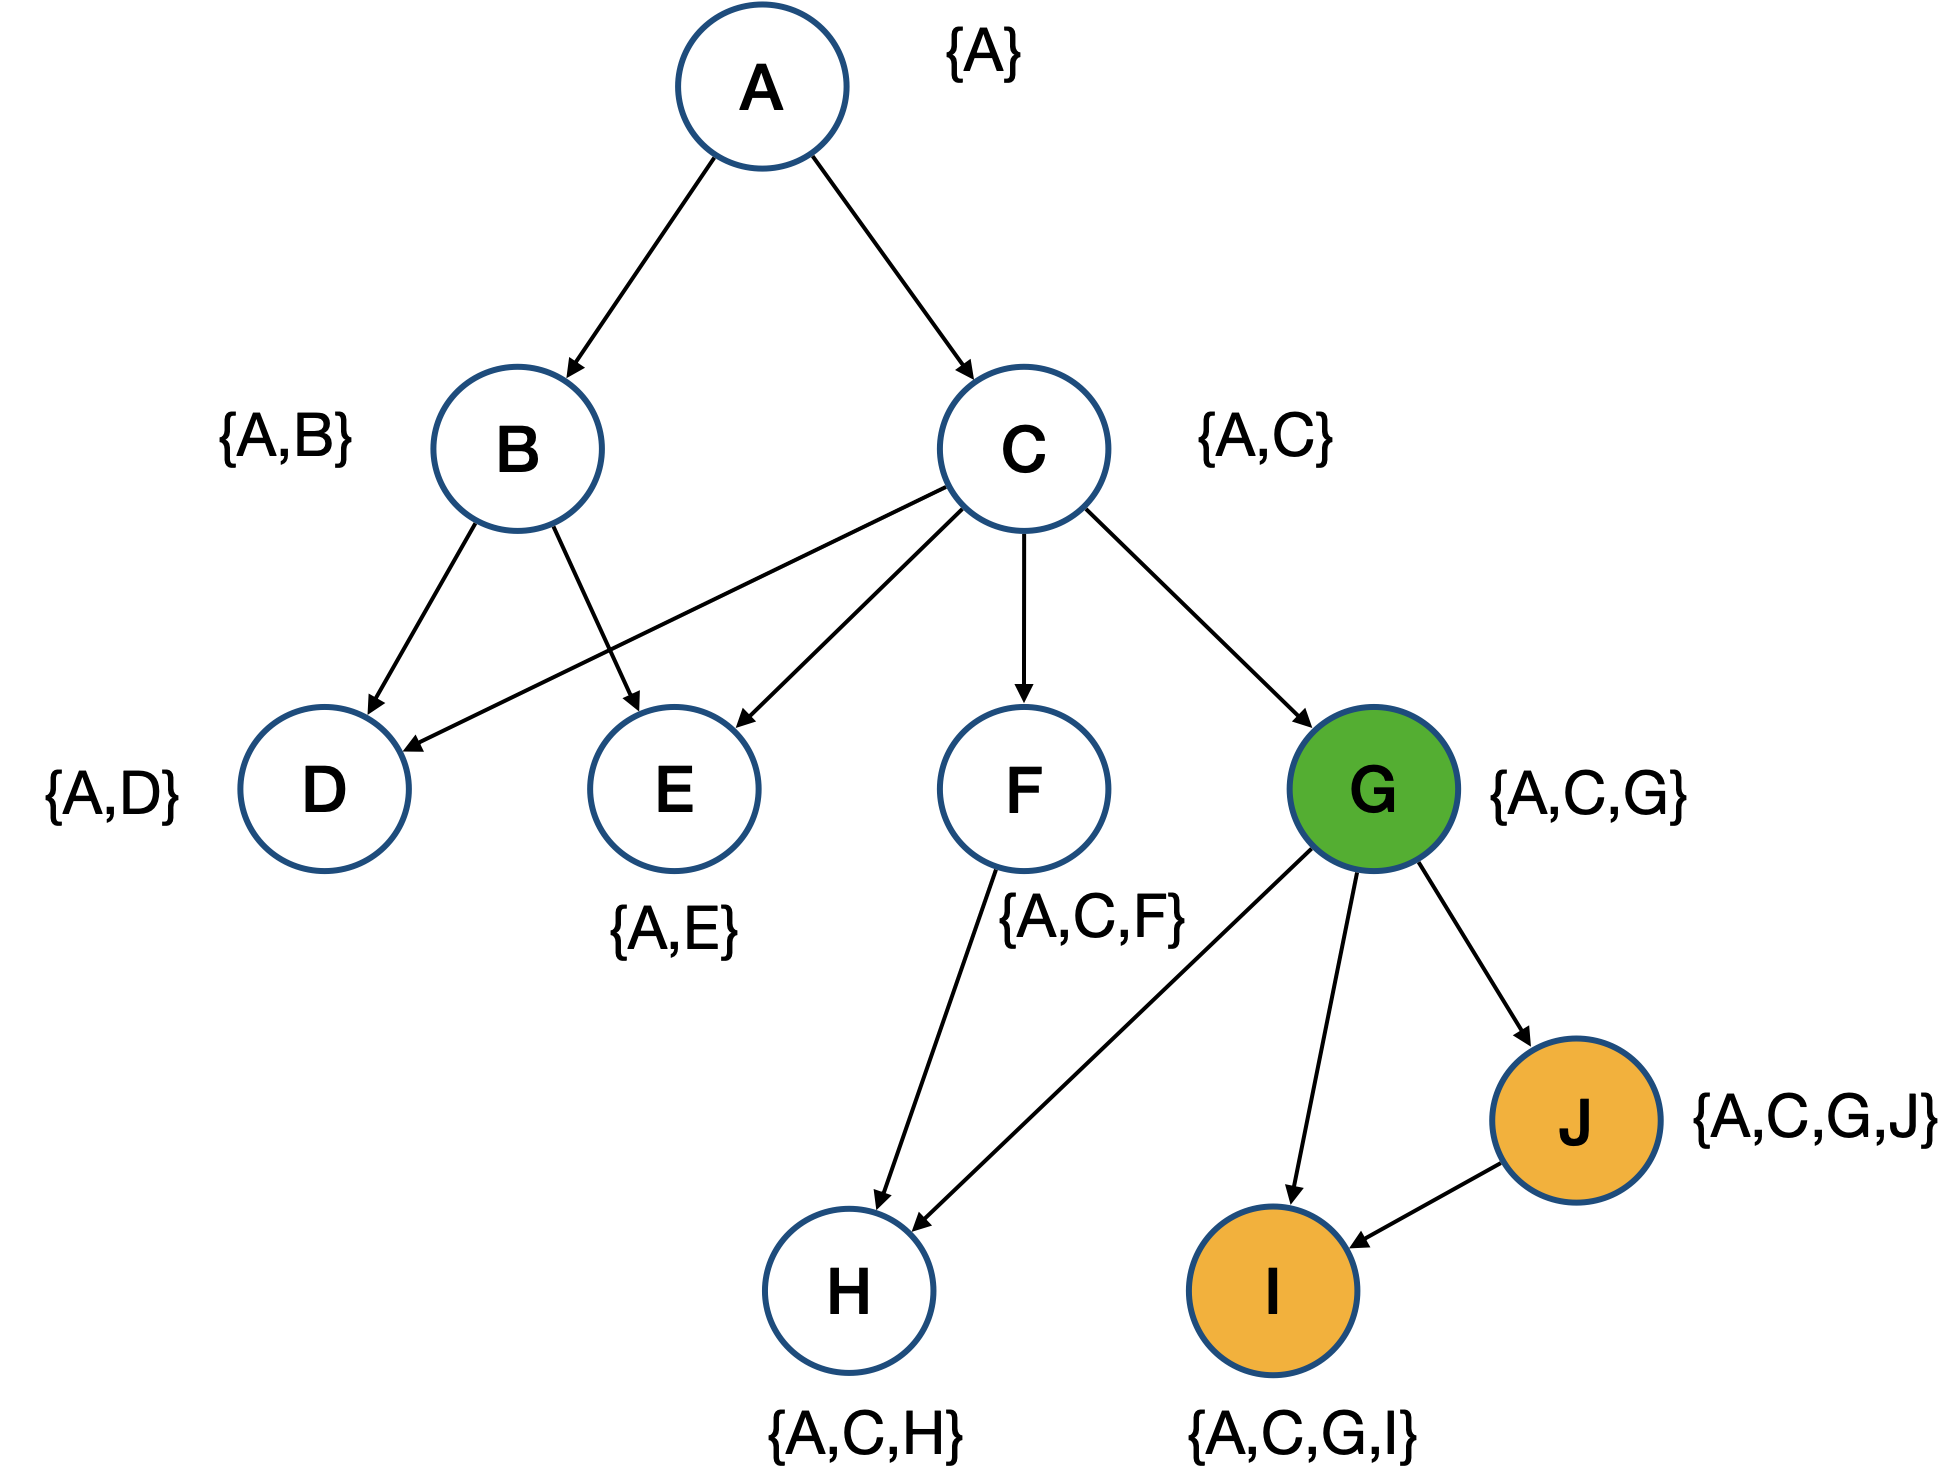
\includegraphics[width=.7\columnwidth]{figures/CALockExample}\\
	{\small
		Lock on G: \{A,C,G\} with grain: \{I, J\}
	}
	\caption{CALock labels}
	\label{calockexample}
\end{figure}

In CALock, when a thread wants to lock a set of lock targets, it issues a lock request for the LGCA of targets, computed by taking a set intersection of their labels (see theorem \ref{proofOfDeepness}). 
This LGCA is a vertex in the graph and is the \emph{guard} for this lock request. A guard is the root of the smallest grain that contains the lock targets. For example, in Figure \ref{calockexample}, to lock I and J, we find their LGCA which is G and place a lock on G (the lock guard).

As soon as the thread identifies the LGCA, it issues a lock request by adding its request to a pool used to identify conflicts (Section \ref{lockPool}). 
The thread then proceeds to check for conflicts and blocks if one exists. In the absence of conflicts, the thread proceeds to its critical section.


\section{Identifying lock conflicts} \label{lockPool}
In MGL on graphs, conflict detection is not as simple as testing for read/write conflicts. Since lock guards have a grain that they protect, it is necessary to ensure that the grain remains exclusive for a writer. With CALock, two conditions indicate a lock conflict. If both conditions hold for a pair of lock requests, they are in conflict. 

\begin{itemize}
	\item The lock requests have a \emph{mode conflict} i.e. a read/write conflict. 
	\item The lock requests have a \emph{grain overlap} i.e. they are trying to lock overlapping grains.
\end{itemize}
Table \ref{compatibilityMatrix} shows compatibility between lock modes.

% \subsection{CALock scheduler}
In order to remain fair and prevent thread starvation, CALock uses sequence numbers to resolve conflicts. The \emph{sequence numbers} are an indication of the order in which the locks are requested. In the presence of conflicts, threads are granted locks in a \emph{First come first serve} order.

A thread that wants to lock a set of targets creates a lock request and adds it to a \emph{lock pool} for conflict detection. 
The request contains the following data.


\begin{itemize}
	\item \textbf{Thread ID}: of the thread requesting the lock
	\item \textbf{Guard ID}: of the vertex being locked in order to lock the set of targets.
	\item \textbf{Guard label}: Label of the lock Guard vertex
	\item \textbf{Sequence number}: allocated to the lock request when it is added to the lock pool.
	\item \textbf{Activity Indicator}: used by other threads to wait in the presence of conflicts.
	\item \textbf{Lock mode}: read or write
\end{itemize}

The lock pool is an array containing one entry per thread. Initially and when the thread is not holding a lock, its entry is \inline|NULL|. 
Algorithm \ref{lockFunction} shows the flow of lock acquisition and conflict detection in the lock pool. 
When a thread arrives in the lock pool with the information of the lock it wants to acquire, it is given a sequence number (line \ref{seqNoAllocation}) and it sets its activity indicator to true (line \ref{waitTrue}) indicating that it is active and using the lock. 
With this additional information, the lock request is added to the pool (line \ref{addToPool}). 
In order to conserve the first come first serve order and prevent race conditions where a later lock request is granted first before the thread with an earlier request could detect the conflict, the three steps involving the assignment of a sequence number, setting the activity indicator and addition to the lock pool are done atomically.

%The sequence number is assigned to the thread before the request is added to the pool. It is used to order the requests by their arrival order. The waiting condition is set to \inline|true| after the sequence number is assigned indicating that the thread is holding the lock. Another thread with conflicting request blocks and waits for this boolean value to change to \inline|false|.

%Assignment of a sequence number, setting the wait condition and addition of the lock request to the pool is done atomically under a mutex to prevent the race where a new lock request with a conflicting operation and grain is granted before the conflict could be detected.

After the lock request is added to the pool, the thread checks for conflicts with other requests in the pool.
\begin{itemize}
	\item \textbf{Mode conflict}: is checked by comparing the lock modes in the requests.
	\item \textbf{Grain overlap}: is checked using the guard ID and guard label of the requests. For two lock requests $R_1$ and $R_2$, if the guard ID of $R1$ is present in the guard label of $R_2$ or vice-versa, then the grains overlap.
	\item \textbf{Arrival order}: If there is a mode and grain conflict, the request with a lower sequence number is granted first.
\end{itemize}

A thread checks these conditions (line \ref{conditionCheck}) by iterating over the pool (line \ref{conflictCheck}). 
When requesting a lock, any thread $T$ can be blocked for a maximum of $n$ turns where $n$ is the maximum number of threads. 
After $n$ blocks, the sequence number of $T$ will be the lowest among all requests in the lock pool and it will be allowed to proceed.
This is essential to prevent thread starvation.

\begin{table}
	\caption{Lock compatibilities between read ($rl$) and write ($wl$) locks requested by threads $i \neq j$ on vertices $x$ and $y$.}
    
    \captionsetup{justification=centering}
		\begin{tabular}{c|cc}
			&$rl_i(x)$   &$wl_i(x)$\\
			\hline
			\rowcolor{gray!20}
			$rl_j(y)$& \ding{51} & \ding{68}\\
			$wl_j(y)$& \ding{68}&\ding{68}\\
		\end{tabular}\\
		\subcaption*{
    	\ding{51} compatible. \\
    	% \ding{55} incompatible.\\
    	\ding{68} compatible iff grain of x is disjoint from grain of y.}
		\label{compatibilityMatrix}
\end{table}



Figure \ref{fig:lockPool} shows the snapshot of a lock pool in use by threads. This pool contains three active threads $T_1, T_2$ and $T_7$. $T_7$ arrives first and is assigned the sequence number 1. $T_1$ and $T_2$ arrive later and have sequence numbers 2 and 3 respectively. 
$T_1$ and $T_2$ conflict because they have overlapping grains. $T_2$ is requesting a lock on C which overlaps with the grain locked by $T_1$. This is detected by checking if C is present in the label of G i.e. $C \in \{A, C, G\}$. To resolve the conflict, $T_1$ is granted a lock since it arrived first and $T_2$ has to wait for $T_1$ to release the lock. $T_7$ does not have a conflict with any thread and acquires a lock on B.

\begin{algorithm}[ht]
	\caption{Lock acquisition request in the lock pool}
	\begin{algorithmic}[1]
		\State $GSeq: $ Global sequence number for lock requests
		\State $Mutex: $ Mutex used when adding requests to the lock pool
		\State $Condition:$ Atomic boolean value used by waiting threads when in conflict
		\Statex

		\Procedure{Lock}{$req$, $threadID$}
		\State \Call{Lock}{$Mutex$}
		\State $req.Seq \gets Gseq++$ \label{seqNoAllocation}
		\State $req.condition.$\Call{TestAndSet}{true} \label{waitTrue}
		\State $Pool[threadId] \gets req$ \label{addToPool}
		\State \Call{Unlock}{$Mutex$}
		\ForAll{ $lock \in Pool \setminus threadID$} \label{conflictCheck}
		\If{ $lock \neq NULL$ \label{conditionCheck} 
			\State $\land(req.\Call{HasRWConflict}{$lock$})$
			\State $\land  (lock.guardID \in req.label \lor  req.guardID \in lock.label)$
			\State $\land (req.Seq > lock.Seq)$ 
		}
		\State $thread.$\Call{BlockAndwait}{$lock.condition$}
		\EndIf
		
		\EndFor
		\State return $true$
		\EndProcedure
		\Statex
		\Procedure{Unlock}{$lock$}
		\State $lockPool.$\Call{Remove}{$lock$}
		\State $lock.condition.$\Call{Clear}{ }
		\State $lock.condition.$\Call{notify\_all}{ }
		\EndProcedure
	\end{algorithmic}
	\label{lockFunction}
\end{algorithm}


\begin{figure*}[ht]
	\centering
	\begin{tikzpicture}[font=\ttfamily,
		array/.style={matrix of nodes,nodes={draw, minimum height=2em, minimum width=\textwidth/10, anchor=center},column sep=-\pgflinewidth, row sep=0.8em, nodes in empty cells,
			row 1/.style={nodes={draw=none, fill=none, minimum size=1em}}}]
		\matrix[array] (array) {
			$T_1$ & $T_2$  &  $T_3$ & $T_4$ &$T_5$  & $T_6$ & $T_7$ \\
			G,read,2,\{A,C,G\}&C,write,3,\{A,C\}&NULL&NULL&NULL&NULL&B,read,1,\{A,B\}\\};

	\end{tikzpicture}
	\caption{Lock pool containing details of locks held by threads}
	\label{fig:lockPool}
\end{figure*}




\section{Structural modifications, locking and relabelling}

CALock can be utilized for static graphs whose structure does not change and for dynamic graphs that change at runtime. 
When a structural modification occurs, the grain in which the modification takes place needs to be relabelled. 
Unlike DomLock, MID and FlexiGran in which the relabelling happens under a global mutex, relabelling in CALock is done under the same lock that is acquired to perform the structural modification. 
Here, we explain the locking and relabelling mechanism for dynamic graphs.

\paragraph*{Vertex addition and deletion}
Adding a vertex to the graph does not change the observable topology because this new vertex is not connected to the graph and hence it is also not reachable from the root. 
So, addition does not require locking or relabelling of any kind. 
Deleting a vertex that does not have any edges does not require synchronization either because a disconnected vertex is not reachable from the root of the graph.

However, to delete a vertex that is reachable from the root i.e. connected to the graph, a lock is required. 
To do this, a write (exclusive) lock is taken on the LGCA of the vertex that needs to be deleted. 
The LGCA guards all the paths reaching this vertex and prevents inconsistent access to it. 
Once the lock is acquired, the vertex is disconnected from the graph and then deleted.

After a vertex is deleted, relabelling might be necessary if the deleted vertex's descendants are still connected to the graph since the set of their ancestors has changed. Relabelling is done by recursively calling the function \inline|BFLabel()| in Algorithm \ref{labelAssignment} on the children of the deleted vertex. 
The lock acquired to delete the vertex is released after the relabelling is complete.

\paragraph*{Edge addition and deletion}
Adding and deleting edges to the graph changes its topology and also the paths to the vertices. 
Both operations are performed under a write (exclusive) lock. 
When adding or deleting an edge between a source vertex $u$ and a target vertex $v$, a write (exclusive) lock is taken on the LGCA of $u$ and $v$. 
Both operations change the ancestors of a vertex so relabelling is initiated at the target ($v$) of the affected edge using \inline|BFLabel()| function in Algorithm \ref{labelAssignment}.

When a vertex has only one incoming edge, deleting that edge disconnects it from the graph. 
In this case, relabelling can be omitted because the target vertex $v$ has no parents and is also not reachable from the root of the graph. 

% \subsection{Relabeling}

% Relabeling involves the same steps as the initial labeling but is performed on the lock grain. This lock grain is a subgraph $G' = (V', E')$ of the graph $G = (V, E)$ such that
% \begin{itemize}
% 	\item $V' \subseteq V$ and $v' = \lvert V' \rvert$
% 	\item $E' \subseteq E \land ((v_1, v_2) \in E' \rightarrow v_1, v_2 \in V')$ and $e' = \lvert E' \rvert$
% \end{itemize}

% In most cases, the complexity of relabeling is proportional to the size of the grain i.e. $\theta(v'+ \frac{v'}{d_{avg}})$.
% In the best case, only a single vertex is locked. So the complexity of relabeling is $\Omega(1)$.
% In the worst case, $G' = G$ i.e. the whole graph is locked.
% This leads to a complexity of $O(2v)$



% \subsection{Conflict detection}
% Detecting lock conflicts involves iterating over a list that contains, at each index, the information of the lock grain.
% The complexity of iterating over the list is $O(n)$ where $n$ is the maximum number of threads.


\section{Properties of CALock} \label{formalProperties}
The properties of any algorithm hold importance in guaranteeing behavioural stability. In this section, we show that CALock is safe, live and does not lead to thread starvation. 
However, it's crucial to emphasize that the discussion of these formal properties only holds true value when the implementation of the locking algorithm is correct. 
CALock requires the assignment of lock request sequence numbers, setting of the activity indicator and addition of the lock pool to happen atomically. 
In our implementation, we use a mutex to achieve this. 
%\subsection[Uniqueness]{Uniqueness}
%
%\paragraph{Property} A thread holds a single lock at a time.
%\paragraph{Discussion} In order to acquire a lock, a thread inserts its request in a lock pool. 
%The pool has a dedicated position where a thread is allowed to insert its request. 
%This prevents threads from inserting multiple requests

\subsection[Safety]{Safety}


\paragraph{Property} A thread holding a write lock on a guard has exclusive access to the corresponding grain. 
This means that when a thread requests a write lock, it is granted the lock only if no other thread can access this grain.

\paragraph{Discussion} By contradiction, assume that two threads $T_1$ and $T_2$ are granted a write lock on the same vertex $v$. 
Then the lock pool would contain, at indices 1 and 2 respectively, two lock requests $R_1$ and $R_2$ with the same lock target $v$ and lock mode $wl$. However, they would have different sequence numbers since sequence numbers are assigned atomically before the requests are added.

At the entry to the critical section, $T_1$ (resp. $T_2$) iterates over the pool to check for conflicts of three kinds (Mode conflict, grain conflict, sequence number conflict). 
Since the iteration is always done in the same order, $T_1$ would detect a mode and grain conflict with $T_2$ and block if its sequence number is higher and vice-versa. 
Hence, $T_1$ and $T_2$ are never, simultaneously granted a lock on $v$. Therefore, CALock is safe.

\subsection[Liveness]{Liveness}
\paragraph{Property} When a thread requests a lock, it is guaranteed to be granted the lock eventually i.e. 
The lock acquisition algorithm does not block forever.

\paragraph{Discussion}
In a correct implementation of an application that uses CALock, when a thread leaves its critical section, it releases the lock it holds and this is guaranteed to happen i.e. threads do not sleep after lock acquisition.  
The lock pool prevents a thread from holding multiple locks. 
If a thread wishes to lock multiple vertices, it requests a lock on their LGCA. 
Since threads hold at most one lock at any given time, deadlocks never occur. 

The absence of deadlocks combined with the guaranteed progress of threads ensures that CALock is live. 

\subsection[Fairness]{Fairness}
\paragraph{Property} When a thread requests a lock, it is granted the lock after a defined number of blocks. 
The lock acquisition algorithm does not lead to a starvation of threads.

\paragraph{Discussion}
CALock uses a FIFO mechanism to grant locks. When a thread is blocked, it is always blocked by a thread that has a lower sequence number. 
A thread can be blocked and bypassed by other threads in the presence of conflicts at most $n$ times ($n$ is the size of the lock pool).  
Since sequence numbers are assigned atomically and are monotonically increasing, a thread is granted its lock after at most $n$ bypasses. 
After a thread is  bypassed $n$ times, the sequence number of that blocked thread would be the lowest and it would be granted the lock it requested. 
This ensures that no thread starves and CALock is fair.


\section{Complexity analysis of CALock} \label{complexityAnalysis}

% \subsection*{Labelling and relabelling}
% \subsection{Labeling of a vertex}
The labeling algorithm involves two operations.
\begin{itemize}
	\item \emph{Traversal}: Recursive BFS over the graph starting from the root. The number of edges examined is dependent on the average degree of vertices. In the worst case, where the graph is complete, the degree of any vertex is the number of vertices in the graph.
	\item \emph{Label computation}: For each vertex, the intersection of its parents' labels needs to be calculated. The number of elements in the label of a vertex is inversely proportional to the number of its parents. A vertex with more parents has more paths from the root and hence, a smaller label. We can approximate this in terms of the vertex degree as well. 
\end{itemize}

For a graph $G = (V, E)$, let $v = \lvert V \rvert$ be the number of vertices, $e = \lvert E \rvert$ be the number of edges and $d_{avg}$ be the average degree of a vertex. According to the Handshake lemma \cite{euler1741solutio}, the average degree of a vertex is 
\begin{equation}
	d_{avg} = \frac{2 \times e}{v} 
\end{equation}

% The maximum size of the label set is $v$; since, for a complete graph, all the vertices will be included in each label at the fix-point.

The complexity of breadth-first traversal is $\theta(v + v.d_{avg})$. 
For each vertex, the size of its label is inversely proportional to the number of parents it has and consequently, label computation is inversely proportional to the average degree i.e. $\theta(\frac{v}{d_{avg}})$. 

The combined complexity of these operations for the initial labeling is $\theta(v^2+ \frac{v^2}{d_{avg}})$.

In the best case, the graph contains only one vertex. The best case complexity is $\Omega(1)$.
In the worst case, the average degree of vertices is 1. Thus, the worst-case complexity is $O(v^2)$.

When a thread requests a lock, it finds the LGCA of the lock targets and issues a lock request. 
The LGCA is computed via a set intersection of the labels of the lock targets. 
If the lock request is for $q$ lock targets and the average label size is $\theta(\frac{v}{d_{avg}})$, the complexity of finding the lock guard is $\theta(\frac{q.v}{d_{avg}})$. Since $q<<v$ for real-world applications, the average case complexity can be reduced to $\theta(\frac{v}{d_{avg}})$. 
In the best case, the lock request is for a single vertex and the complexity is $\Omega(1)$. In the worst case, the lock request is for all vertices of the graph and the complexity is $O(\frac{v^2}{d_{avg}})$.


These labels are then used to detect conflicts. A thread checks conflicts with all other threads i.e. $n$ times. For each conflict, a set membership test is performed. With an efficient set implementation, the membership can be tested in $O(1)$. The complexity of conflict detection is $\theta(n)$.

\begin{table}
	\centering
	\captionsetup{justification=centering}
	\begin{tabular}{l | cccc}
				 		& Labelling 								&	Relabelling 		& Lock Guard computation 						& Conflict detection\\
						\hline
		DomLock 		& $\theta(v^2+ \frac{v^2}{d_{avg}})$ 		&					& $\theta(v^2+ \frac{v^2}{d_{avg}})$			& $O(n)$\\
		MID 			& $\theta(2v^2+ \frac{2v^2}{d_{avg}})$ 		&					& $\theta(v^2+ \frac{v^2}{d_{avg}})$ 			& $O(n)$\\
		FlexiGran 		& $\theta(v^2+ \frac{v^2}{d_{avg}})$		&					& $\theta(v^2+ \frac{v^2}{d_{avg}})$  			& $O(n)$\\
		CALock 			& $\theta(v^2+ \frac{v^2}{d_{avg}})$ 	 	&					& $\theta(\frac{v}{d_{avg}})$ 					& $O(n)$
	\end{tabular}\\
	\caption{Average case complexities of MGL techniques}
\end{table}

\begin{table}
	\centering
	\captionsetup{justification=centering}
	\begin{tabular}{l | cccc}
				 		& Labelling 					&Relabelling			& Lock Guard computation 			& Conflict detection\\
						\hline
		DomLock 		& $\theta(v^2)$ 				&						& $\theta(v^2)$						& $\theta(n)$\\
		MID 			& $\theta(2v^2)$ 				&						& $\theta(v^2)$ 					& $\theta(n)$\\
		FlexiGran 		& $\theta(v^2)$					&						& $\theta(v^2)$  					& $\theta(n v^2)$\\
		CALock 			& $\theta(v^2)$ 	 			&						& $\theta(1)$ 						& $\theta(n)$
	\end{tabular}\\
	\caption{Worst case complexities of MGL techniques}
\end{table}


% \begin{table}[ht]
%     \centering
% 	\captionsetup{justification=centering}
% 	\caption{Time complexities of the operations in MGL techniques}
% 	\begin{tabular}{l c c}
% 		&Average Case & Worst case\\
% 		\hline
% 		DomLock Labelling 					& $\theta(v^2+ \frac{v^2}{d_{avg}})$ 						& $O(v^2)$\\
% 		DomLock Dominator computation 		& $\theta(v^2+ \frac{v^2}{d_{avg}})$ 						& $O(v^2)$\\
% 		DomLock Conflict detection 			& $\theta(n)$ 												& $O(n)$\\
% 		\hline
% 		MID Labelling 						& $\theta(2v^2+ \frac{2v^2}{d_{avg}})$ 						& $O(2v^2)$\\
% 		MID Dominator computation 			& $\theta(v^2+ \frac{v^2}{d_{avg}})$ 						& $O(v^2)$\\
% 		MID Conflict detection 				& $\theta(n)$ 												& $O(n)$\\
% 		\hline
% 		FlexiGran Labelling 				& $\theta(v^2+ \frac{v^2}{d_{avg}})$ 						& $O(v^2)$\\
% 		FlexiGran Dominator computation 	& $\theta(v^2+ \frac{v^2}{d_{avg}})$ 						& $O(v^2)$\\
% 		FlexiGran Conflict detection 		& $\theta(n)$ 												& $O(n)$\\
% 		\hline
% 		CALock Labelling 					& $\theta(v^2+ \frac{v^2}{d_{avg}})$ 						& $O(v^2)$\\
% 		CALock LGCA computation 			& $\theta(\frac{s.v}{d_{avg}})$ 							& $O(\frac{v^2}{d_{avg}})$\\
% 		CALock Conflict detection 			& $\theta(n)$ 												& $O(n)$
% 		% Relabeling &  $\theta(v'+ \frac{v'}{d_{avg}})$ & $\Omega(1)$ & $O(2v)$
% 	\end{tabular}\\
	
% 	\label{timecomplexity}
% \end{table}
